\section{Activities}

\begin{frame}[c,fragile]
	\frametitle{Swing Button App}
	\begin{columns}
	\column{.7\textwidth}
	\begin{lstlisting}
	public static void main(String[] args) {
	    JFrame myFrame = new JFrame();
	    myFrame.addComponent(
	        new JButton("Click me!"));
	    myFrame.show();
	    ...
	}
	\end{lstlisting}

	\pause
	\column{.3\textwidth}
	\vspace{1cm}
	\begin{figure}
	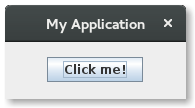
\includegraphics[width=3cm]{pictures/button-swing.png}
	\end{figure}
	\end{columns}

	\pause \vspace{0.5cm}
	\begin{figure}
	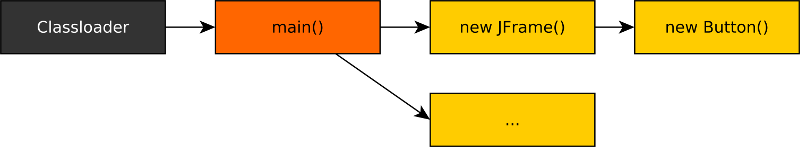
\includegraphics[width=\textwidth]{pictures/call-hierachy-swing.png}
	\end{figure}
\end{frame}


\begin{frame}[c]
	\frametitle{Android App}
	\begin{columns}[t]
	\column{.7\textwidth}
	\begin{itemize}
	\item nur ein Fenster kann angezeigt werden \pause
	\item weniger Prozessor- und Akkuleistung \pause \\
		$\Rightarrow$ System muss mit Resourcen haushalten \pause
	\item stärkere Systemintegration \\ (Notifications, Sensoren,...) \pause
	\end{itemize}
	\vspace{0.2cm}
	$\Rightarrow$ \textbf{Activities} \\
	\hspace{1cm}Container für graphische Anwendungen \pause

	\column{.3\textwidth}
	\vspace{-1cm}
	\begin{figure}
	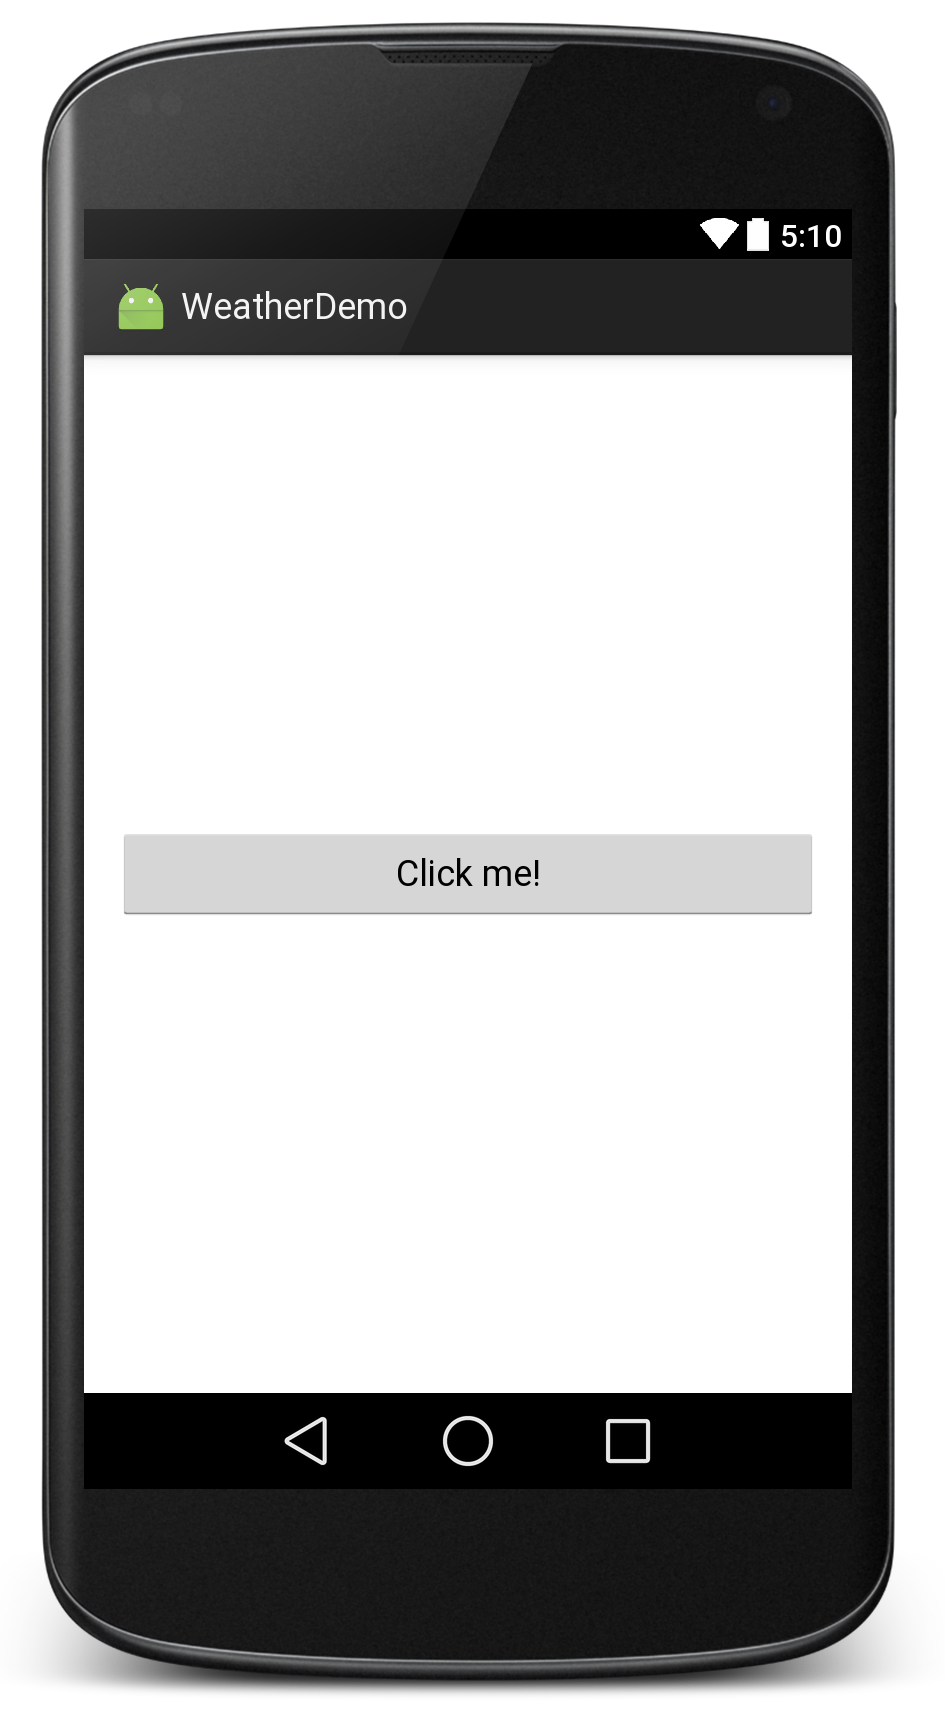
\includegraphics[height=6cm]{pictures/button-android-framed.png}
	\end{figure}
	\end{columns}
\end{frame}

\begin{frame}[c,fragile]
	\frametitle{Android Button App}
	\begin{lstlisting}
	class MainActivity extends Activity {
	    @Override
	    public void onCreate() {
	        //TODO add Button
	    }
	}
	\end{lstlisting}
	\pause \vspace{0.5cm}
	\begin{lstlisting}[language=XML]
	<manifest>
	  <application label="ButtonApp">
	    <activity name=".MainActivity" 
	              label="My Activity">
        ...
	</...>
	\end{lstlisting}
\end{frame}

\frame[c]{
	\frametitle{Inversion of control}
	\centering
	\textbf{Swing}
	\begin{figure}
	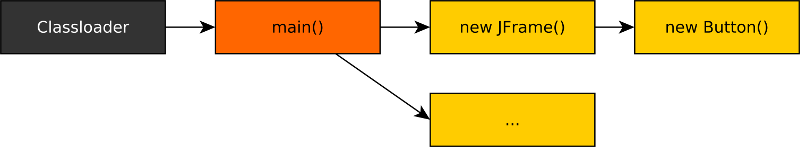
\includegraphics[width=0.8\textwidth]{pictures/call-hierachy-swing.png}
	\end{figure}
	\vspace{0.2cm}\pause
	\textbf{Android}
	\begin{figure}
	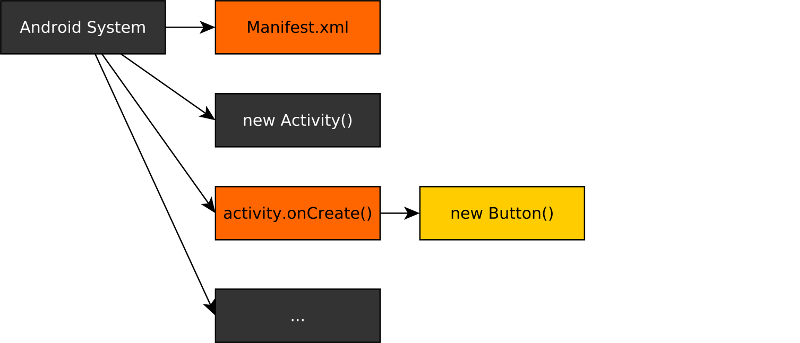
\includegraphics[width=0.8\textwidth]{pictures/call-hierachy-android.png}
	\end{figure}
}

\frame[c]{
	\frametitle{Activity Lifecycle}
	\begin{figure}
	\centering
	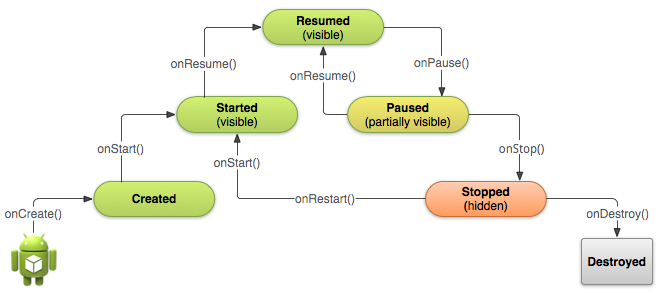
\includegraphics[width=\textwidth]{pictures/activity_lifecycle.png}
	\end{figure}
	\pause
	\begin{columns}
	\column{.5\textwidth}
	\textbf{onCreate()}
	\begin{itemize}
	\item initialize UI \pause
	\item start Animations \pause
	\item connect to Sensors \pause
	\end{itemize}
	\column{.5\textwidth}
	\textbf{onDestroy()}
	\begin{itemize}
	\item persist User Data \pause
	\item stop Animations \pause
	\item disconnect from Sensors
	\end{itemize}
	\end{columns}
}

\frame[t]{
	\frametitle{Intents...}
	\begin{itemize}[<+->]
		\item Hauptkommunikationsmittel zwischen Komponenten
		\item ... enthalten explizites oder implizites Ziel \\
			\textit{z.B. ``Öffne Facebook'' oder ``Sende Mail''}
		\item ... können noch weitere Daten enthalten \\
			\textit{z.B. Titel der Mail, URL einer Website, ...}
		\item ... werden vom System an das jeweilige Ziel weitergeleitet
	\end{itemize}
	\vspace{-0.5cm}
	\begin{columns}
	\column{.2\textwidth}
	\column{.3\textwidth}
	\begin{figure}
	\includegraphics[height=3cm]<5->{pictures/implicit-intent-hierarchy.pdf}
	\end{figure}
	\pause
	\column{.3\textwidth}
	\begin{figure}
	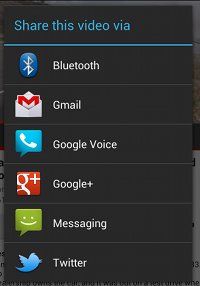
\includegraphics[height=3cm]{pictures/intent-choser.png}
	\end{figure}
	\column{.2\textwidth}
	\end{columns}
}